\documentclass{article}

\usepackage{enumerate}
\usepackage{amssymb}
\usepackage{amsmath}
\usepackage{algorithm}
\usepackage[noend]{algpseudocode}
\usepackage{graphicx}
\usepackage{listings}

\graphicspath{ {Images/} }

\topmargin=-0.45in
\evensidemargin=0in
\oddsidemargin=0in
\textwidth=6.5in
\textheight=9.0in
\headsep=0.25in

\title{CS 189: Homework 3}
\author{Michael Stephen Chen\\ Kaggle Acct: michaelstchen \\SID: 23567341}

\begin{document}
\maketitle

\pagebreak

\section*{Problem 1}
\begin{enumerate}[a)]
  \item
  \item
\end{enumerate}

\section*{Problem 2}
Below are my isocontour plots for part a-e
\begin{center}
  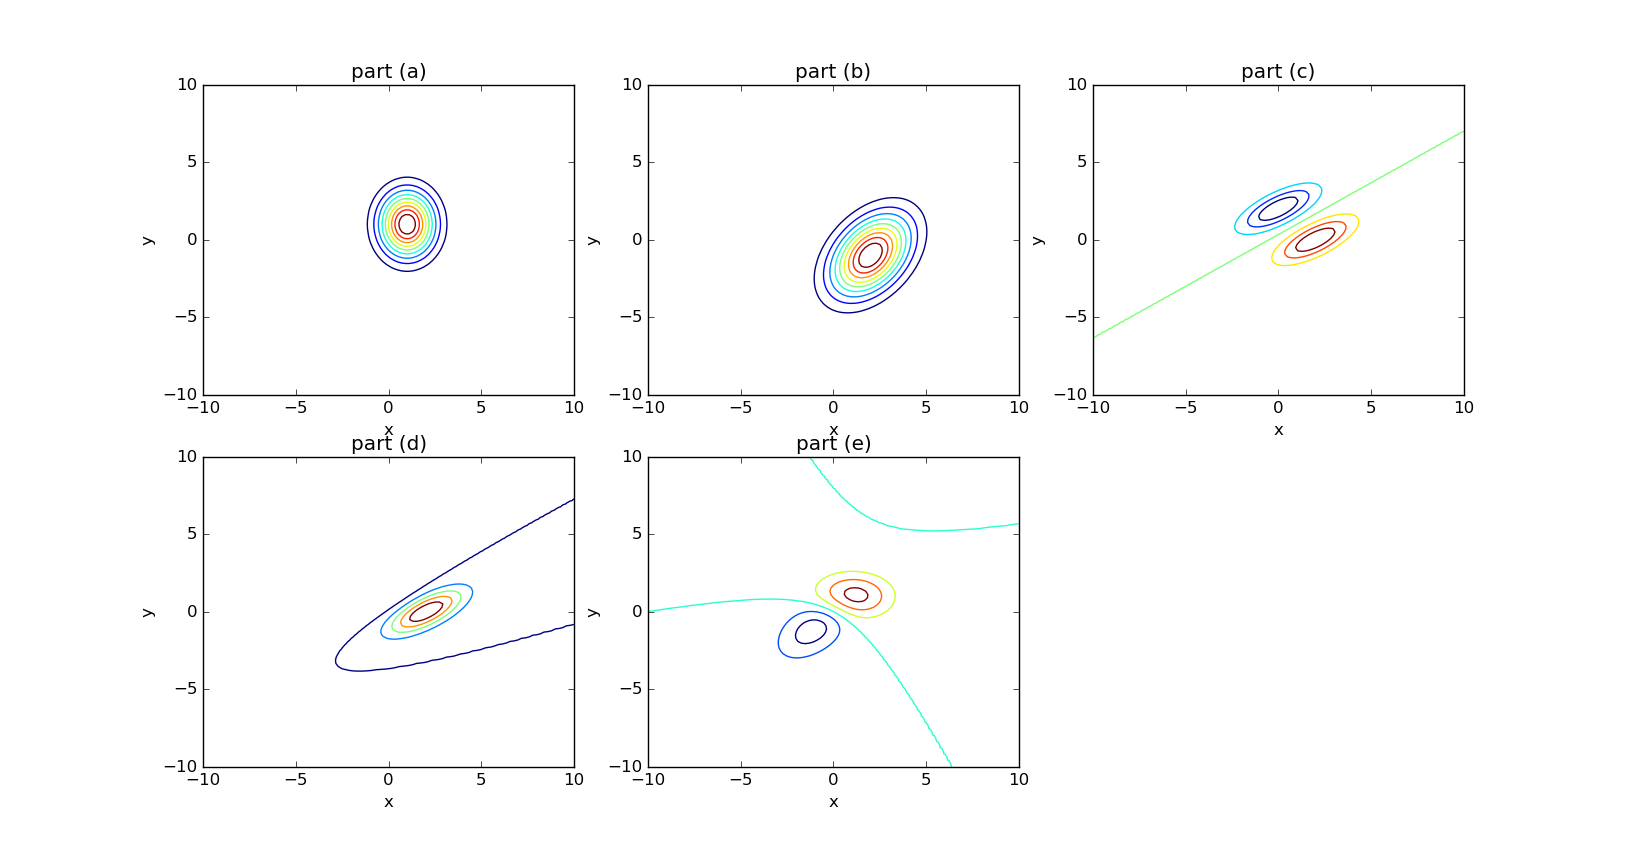
\includegraphics[scale=0.4]{prob2}
\end{center}


\section*{Problem 3}
\begin{enumerate}[a)]
  \item For one run I found the mean to be $mean^T = \left[2.926, 5.776\right]$, which is close to what we expect of $\mu^T = \left[3, 5.5\right]$ if we took an infinite number of samples. Please see the variable \textit{mu} in the file \textit{prob3.py}
  \item Please see the variable \textit{covmat} in the file \textit{prob3.py} for my covariance matrix.
  \item Please see the variables \textit{eigvals} and \textit{eigvecs} in the file \textit{prob3.py} for my eigenvalues and eigenvectors, respectively.
  \item Below is my plot of the $X_1$ and $X_2$ samples in blue, the mean in red, and the eigenvectors of the covariance matrix as arrows
    \begin{center}
      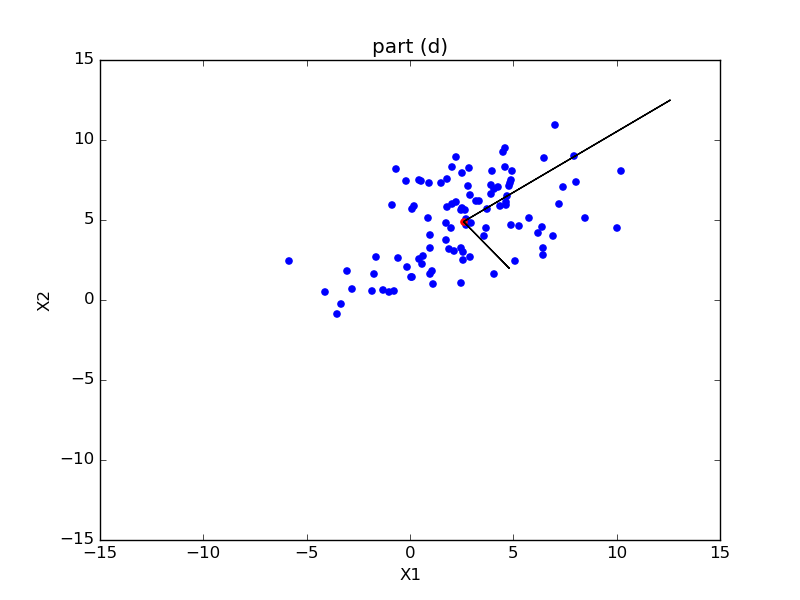
\includegraphics[scale=0.5]{prob3d}
    \end{center}
  \item Below is my rotated plot of the $X_1$ and $X_2$ samples so that the eigenvectors of the covariance matrix correspond to the axes.

    \begin{center}
      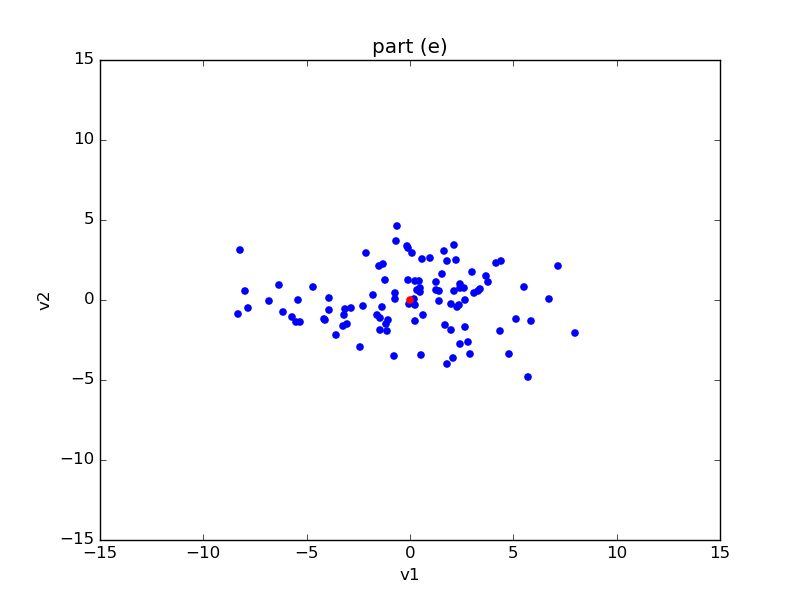
\includegraphics[scale=0.5]{prob3e}
    \end{center}

\end{enumerate}


\section*{Problem 4}
\begin{enumerate}[a)]
  \item
  \item
  \item
  \item
\end{enumerate}


\section*{Problem 5}
\begin{enumerate}[a)]
  \item The MLE for the mean ($\hat{\mu}$) is simply the sample mean for our samples $x_i$
    $$\hat{\mu} = \frac{1}{n} \sum\limits_{i=1}^n x_i$$
    The MLE for the covariance matrices is simply a square matrix with the variances of the features along the diagonal and zeros on the off-diagonals. This is because we assume the features to be i.i.d, meaning that they are independent of one another. As a result the $Cov(X_i, X_j) = 0$ if $i \neq j$. These make up the off-diagonals. When $i=j$, $Cov(X_i, X_j) = Var(X_i)$, which will be the diagonals for our covariance matrix. See \textit{prob5abc.py}.
  \item We can model the prior distribution for each class by tabulating the counts of each digit sample in our training set data and dividing by the total number of samples. So we essentially compute the percent composition of each class in the training set and use that as an estimate for our class priors. See \textit{prob5abc.py}.
  \item Below are the visualizations for the ``0" and ``1" covariance matrices

    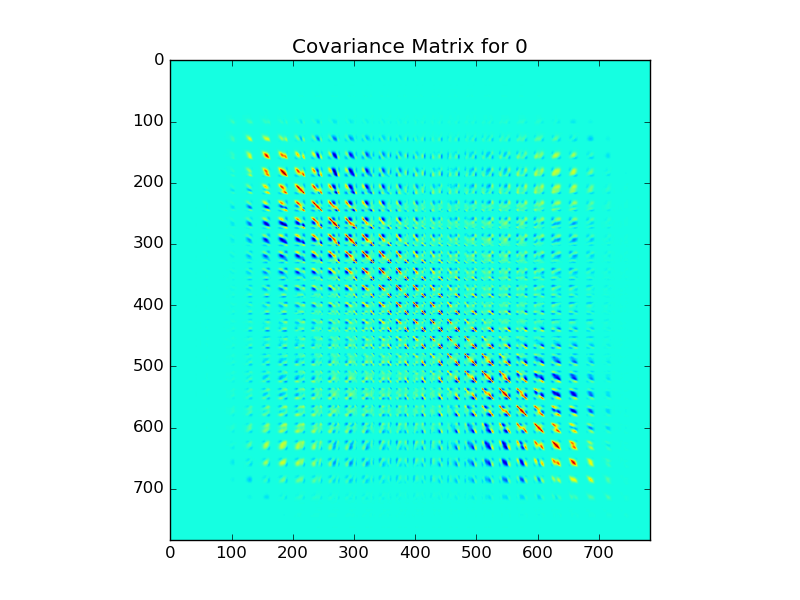
\includegraphics[scale=0.4]{prob5c0}
    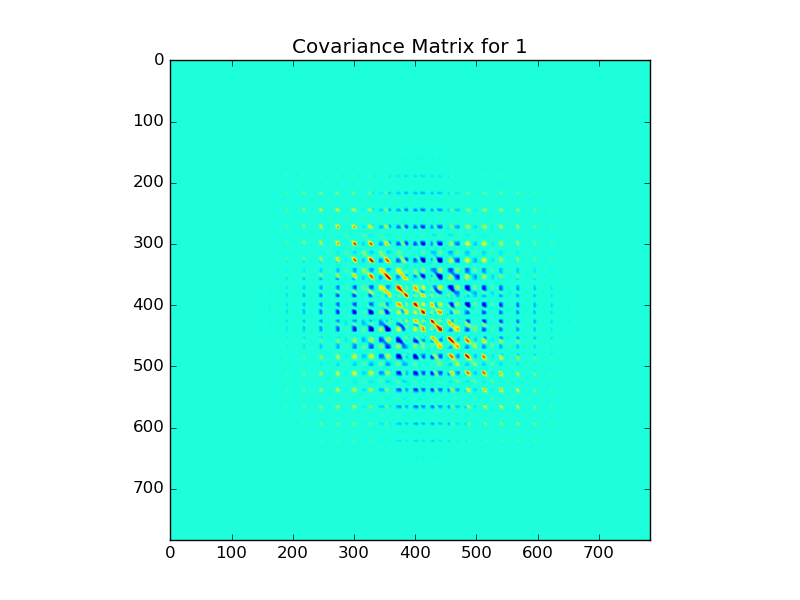
\includegraphics[scale=0.4]{prob5c1}

    The axes are the features. The light blue regions represent relatively independent features while the redder regions represent regions that are highly dependent.

  \item Below is a plot of error rate vs sample size for our LDA digits classifier
    \begin{center}
      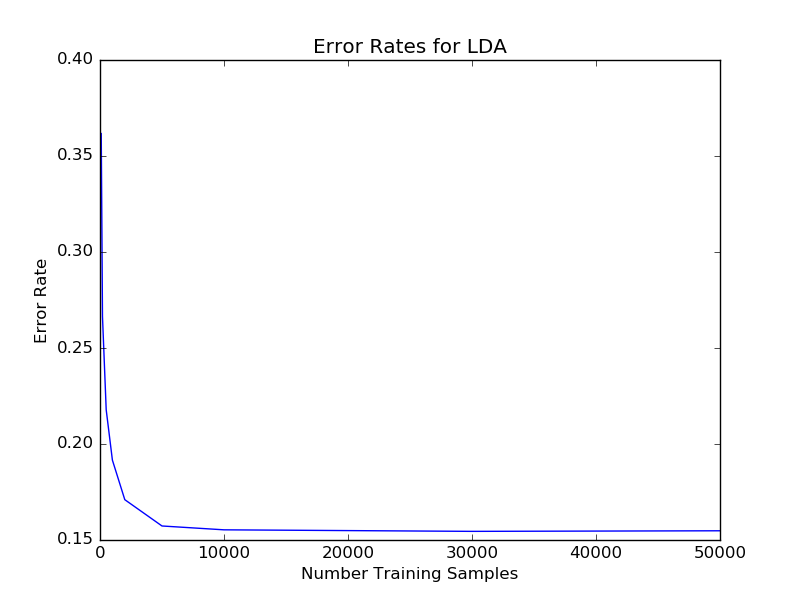
\includegraphics[scale=0.5]{prob5di}
    \end{center}
    The error rates are as follows:
    \begin{center}
      $\begin{array}{c|c}
        Sample Size & Error Rate \\ \hline
        100 &  0.3617\\
        200 &  0.2664\\
        500 &  0.2178\\
        1000 &  0.1916\\
        2000 & 0.1710\\
        5000 & 0.1573\\
        10000 & 0.1553\\
        30000 & 0.1545\\
        50000 & 0.1548
      \end{array}$
    \end{center}
    When we use just one overall covariance matrix, the discriminant function (our decision boundaries) turn out to be linear:
    $$\mu_c^T \Sigma^{-1}x - \frac{1}{2}\mu_c^T\Sigma^{-1}\mu_c + ln(\pi_c)$$

  \item Below is a plot of error rate v sample size for our QDA digits classifier
    \begin{center}
      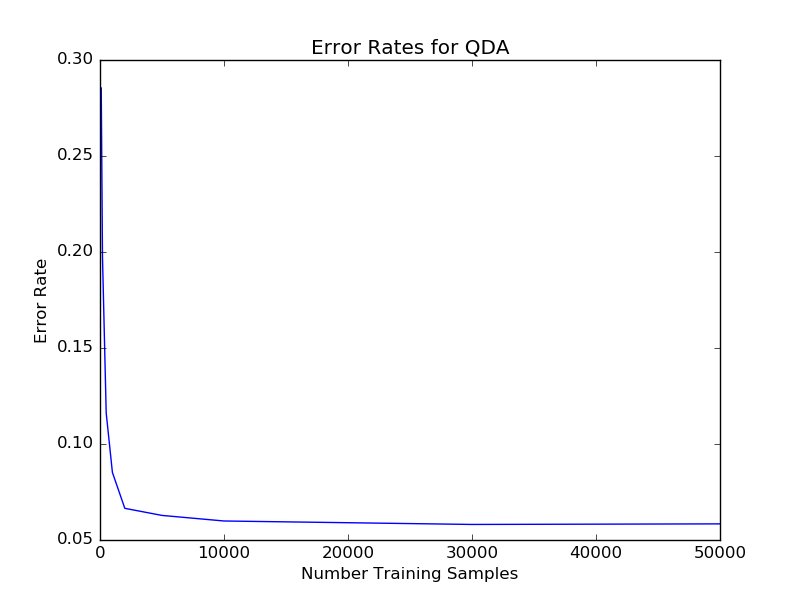
\includegraphics[scale=0.5]{prob5dii}
    \end{center}
    The error rates are as follows:
    \begin{center}
      $\begin{array}{c|c}
        Sample Size & Error Rate \\ \hline
        100 & 0.2854\\
        200 & 0.1976 \\
        500 & 0.1161 \\
        1000 & 0.0852 \\
        2000 & 0.0665\\
        5000 & 0.0628\\
        10000 & 0.0599\\
        30000 & 0.0581\\
        50000 & 0.0584
      \end{array}$
    \end{center}
    When we use a covariance matrix for each class, the disscriminant function (our decision boundaries) turn out to be quadratic:
    $$-\frac{1}{2}(x-\mu)^T \Sigma_c^{-1}(x-\mu) - \frac{1}{2}ln|\Sigma_c| + ln(\pi_c)$$

  \item The LDA classifier's performances were lower than the QDA's probably because the LDA is underfitting the data because it only uses an average, overall covariance matrix.

  \item When I train all all 60000 training samples and classify the 10000 test samples using the QDA procedure, I get a accuracy of 0.93620. I did not use any additional features.

  \item Using the QDA method, this time with the multivariate\_normal.logpdf() function to determine the discriminant, I got an accuracy of 0.79834. For some reason I was trending around 0.59 when I sued the same QDA implementation from the previous part but I get a much higher score with this. I was reading that multivariate\_normal.logpdf uses the pseudoinverse so maybe that's why. I added some additional feature words in \textit{featurize.py} (e.g. ``penis").
\end{enumerate}


\section*{Problem 6}
\begin{enumerate}
  \item Please see \textit{prob6.py}
  \item My residual sum of squares for my 1200 training sample data was 5794953797667.3555. The predicted range of home values is [-56562.83, 710798.84]. The minimum definitely doesn't make sense given that you can't have a negative home value (debt?). The max seems reasonable, especially here in the bay area, but is significantly higher that the actual max of the validation set (5000001)
  \item Below is a plot of my regression weights for all terms except the constant term
    \begin{center}
      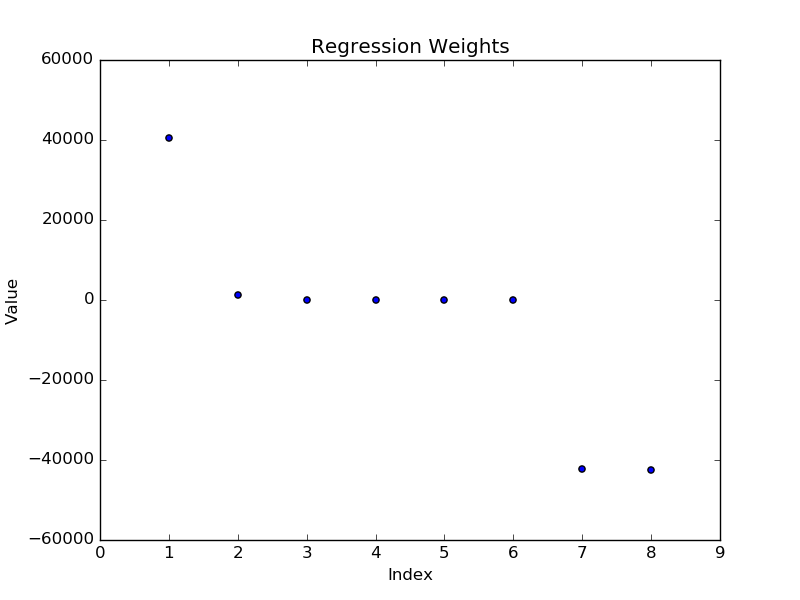
\includegraphics[scale=0.5]{prob6_3}
    \end{center}
  \item Below is a histogram of my training data residuals. It resembles a normal distribution, albeit a little skewed.
    \begin{center}
      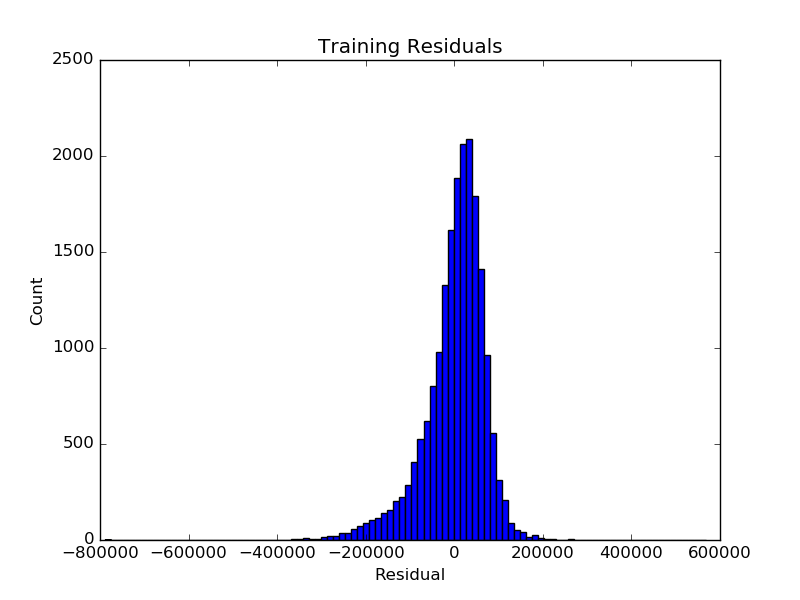
\includegraphics[scale=0.5]{prob6_4}
    \end{center}
\end{enumerate}

\pagebreak

\section*{Appendix: prob2.py}
\lstinputlisting[language=python]{prob2.py}



\section*{Appendix: prob3.py}
\lstinputlisting[language=python]{prob3.py}



\section*{Appendix: prob5di.py}
\lstinputlisting[language=python]{prob5di.py}



\section*{Appendix: prob5dii.py}
\lstinputlisting[language=python]{prob5dii.py}



\section*{Appendix: prob5div.py}
\lstinputlisting[language=python]{prob5div.py}



\section*{Appendix: prob5e.py}
\lstinputlisting[language=python]{prob5e.py}



\section*{Appendix: prob6.py}
\lstinputlisting[language=python]{prob6.py}


\end{document}
